\documentclass[runningheads]{llncs}
%
\usepackage[T1]{fontenc}
\usepackage{graphicx}
% If you use the hyperref package, please uncomment the following two lines
% to display URLs in blue roman font according to Springer's eBook style:
%\usepackage{color}
%\renewcommand\UrlFont{\color{blue}\rmfamily}
%
\begin{document}
%
\title{\large Report on "Theory of Mind May Have Spontaneously Emerged in Large Language Models" \\
\normalsize Paper Report as Part of the "Current Topics of Computational Social Science" Seminar}

%
\titlerunning{Report on "ToM May Have Spontaneously Emerged in LLMS"}
% If the paper title is too long for the running head, you can set
% an abbreviated paper title here
%
\author{Taline Kehlenbach}
%
\authorrunning{T. Kehlenbach}
% First names are abbreviated in the running head.
% If there are more than two authors, 'et al.' is used.
%
\institute{RWTH Aachen}
%
\maketitle              % typeset the header of the contribution
%
\begin{abstract}
This report summarises, questions and critisises the paper "Theory of Mind May Have Spontaneously Emerged in Large Language Models" by Kosinski

\keywords{Artificial Intelligence  \and Theory of Mind \and Language Model}
\end{abstract}
%
%
%

\section{Introduction}
%this section should introduce the paper and ist goals.

Theory of Mind is known in psychology as the ability to understand and reason about one's own and other individual's mental states such as differing beliefs or knowledge states \cite{theory_of_mind}. Most importantly, ToM is regarded to be a uniquely human ability \cite{tom_in_animals}. The research presented in the paper titled "Theory of Mind May Have Spontaneously Emerged in Large Language Models" attempts to contradict this understanding and suggests that large language models may already possess Theory of Mind while not being specifically designed to solve problems for which Theory of Mind is needed. By conducting three studies on the reasoning capabilities of large language models (LLM) such as GPT-3 and GPT-4 Kosinski attempts to prove this hypothesis and compares the results to research on Theory of Mind in developmental psychology, giving an interesting insight in the status of Artificial Intelligence compared to human intelligence.

\section{Related Work}
%it summarizes the state of the art. Puts the paper in context.
\subsection{Theory of Mind}
While Theory of Mind and the research related to it in a purely psychological understanding is more of a foundation for the paper in question it is still important to know what the term means and the research it is related to, to grasp the context of the paper at hand.

Theory of Mind encompasses all abilities that infer various mental states based on contextual information. The term Theory of Mind (ToM) gained traction in the late 1970s and has since found firm footing in developmental psychology where the term is used to determine the existence and emergence of ToM in children. ToM is also a key part to enable predictions of behaviour based on someone's mental state.\cite{theory_of_mind}

The research around ToM in child development plays an important role in Kosinski's work since he uses both well-cited methods and results from this field to first construct ToM tests for LLMs and consecutively compares the LLMs' performances to that of children in different age groups. Therefore, the relevant methods and research results will be shortly surmised in the following. In order to assess a child's ability to differentiate reality from beliefs, false-belief tests were introduced by several researchers \cite{fb_test_places_1,fb_test_places_2,fb_test_contents}. In theses tests children were exposed to situations in which they have to make distinctions between reality and the knowledge or belief of another person about reality and predict someone's behaviour according to it. Kosinskis work is based on two kinds of these tests.

First, the Smarties Task developed by Perner et al. in 1987. In this experiment children around age 4 are shown a tube of "Smarties" (chocolate candy), asked its contents and then shown the real contents which were actually random objects and not candy. They would then be asked the questions what another child who did not see the real contents of the tube would expect to be inside, thus testing the reasoning skills about false beliefs of others. \cite{fb_test_contents}

Second, the Sally-Anne Task first used in a study from 1983 \cite{fb_test_places_1} and then again in 1985 \cite{fb_test_places_2} (this time coining the name Sally-Anne Task) tests the same reasoning ability of attributing false beliefs to others. In this task two agents are introduced (typically using puppets). One agent places an item and leaves the scene while the other agent moves the item before the first agent comes back to look for the item. The children are then asked about the expected behaviour of the first agent who did not witness the displacement of the item. The task is solved correctly when the child predicts that the first agent will search the item in the place where they left it before the second agent moved it, thus proving the child's ability to infer false beliefs of other people. \cite{fb_test_places_1,fb_test_places_2}

In alignment with Kosinski's paper the Smarties Task will be called Unexpected Contents Task and the Sally-Anne task will be called Unexpected Transfer Task as a generalisation and for better understanding of the terms.

As for results in developmental psychology regarding ToM, Kosinski refers to the work of Wellman et al. which agglomerates several studies on ToM (and other attributes) of children mainly aged from 2.5 to 6 years old and interpolates their performance on both Smarties and Sally-Anne Tasks \cite{tom_children_2001}. The results of this paper are used to compare the performance of LLMs on similar tasks to the performance of children in an attempt to assign an age to the level of reasoning LLMs supposedly posses.

Finally, it is important to note that these tests though well-established do not cover the whole landscape of ToM testing that currently exists. There is the Faux-Pas Test for social intelligence \cite{tom_test2} or the Reading-the-Mind-in-the-Eyes Test to test emotional intelligence in adults \cite{tom_test1}. These tests are not taken into account in Kosinski's research.

\subsection{Large Language Models}
The second foundational knowledge related to Kosinski's paper is that about Large Language Models (LLMs). Therefore, in this section some key facts about LLMs and specifically GPT-1 to GPT-4 are presented since these models are used in Kosinski's paper.

LLMs are used in the field of Natural Language Processing (NLP) for text generation, question answering or other text-related tasks that they can be fine-tuned to do. The underlying architecture most frequently used is a Transformer which revolutionised deep learning techniques when it was introduced in 2017 \cite{attention}. Transformers in NLP get a tokenised version of the input text and output probabilities for each word of the vocabulary for the output text generation. The most important part here is that during training the Transformer trains an Attention layer, which can basically learn contextual relations of words.

For LLMs as the name suggests the trainable parameters reach very high numbers (up to several billions). The models are pre-trained on a large text databases and can be fine-tuned on specific tasks to create custom models. Generative Pre-Trained Transformers (GPT) first got published by OpenAI in 2018 with GPT-1 which had a parameter size of approximately 110 million and pre-trained on roughly 7,000 books \cite{gpt1}. Since then the model got developed further and over several iterations and grew both in parameter size and training data. GPT-3 already has 175 billion parameters and was only published two years later \cite{gpt3}.

An interesting characteristic of LLMs compared to smaller language models is that they develop skills as byproducts \cite{llms}. LLMs are mostly trained on completing text prompts and no other abilities are specifically engineered into their architecture, so any other ability like translating text or reading comprehension spontaneously emerge. LLMs also seem to be so-called few-shot learners. This means that no extensive fine-tuning is needed to teach a new task to a pre-trained LLM but rather few training examples suffice for the LLM to be able to perform well on the given task compared to other state-of-the-art-models. They even perform well in zero-shot experiments where the model was given no prior example of the task at hand and used solely in its pre-trained form. \cite{gpt3}

\subsection{Theory of Mind in Large Language Models}
As for the combination of the topics above: Theory of Mind in Large Language Models and the research regarding this field should be discussed. A paper published a few months before Kosinski's take on this topic suggests that LLMs do not possess ToM. The presented experiments consist of tests using GPT-3 both in pre-trained form and few-shot form. The datasets used are SocialIQa probing emotional and social intelligence \cite{socialiqa} and ToMi QA \cite{tomi} which contains false-belief tests resulting in almost 4,000 questions asked for each model. The results of this method show that GPT-3 at the time has below 60\% accuracy in one-shot applications and reaches 60\% accuracy given 24 training examples i.e. up to 24 "shots" before solving the task and thus perform far below humans. \cite{related}

Other papers relating to Kosinski's work will be discussed in later sections of this report as they are more recent than the paper in question, follow up on the research presented and therefore are easier to put into context once the methods and results of Kosinski have been explained in the sections coming up.

\section{Methods}
%this section explains how the problem is approached, which techniques are used and why these ones and not others.
\subsection{Overall Methods}

\subsection{Study 1}

\subsection{Study 2}

\subsection{Study 3}

\section{Results and Discussion}
%in this section, the results of the research are presented, and how they are related to the problem under study and to what it was known until date.
\subsection{Results of Studies 1-3}
The results of the first and second study show that GPT-3.5 correctly answers the two example tasks with almost 100\% probability for choosing the correct answer in each prompt. Furthermore the development of answer probabilities following each sentence of the task descriptions aligns with the answers expected by the author given the amount of information given for each prompt e.g., in the Unexpected Contents Task the prediction of the correct content does not change even when the faulty label is introduced however the prediction of belief switches from the actual content to the one described on the label as the fact that the actual contents are unknown and imperceivable to the person is introduced. It is interesting to not that the prompts regarding the actual state of reality in both tasks are always answered with 100\% certainty whereas the prompts regarding false beliefs almost always have a probability below 100\% and go as low as 82\% in one case. As for the results using scrambled versions of the tests the model only solved 6\% of the Unexpected Contents Tasks and 11\% of the Unexpected Transfer Tasks correctly, proving that the order of the information is crucial for the model's ability to pass the chosen tests.

Regarding study 3 the results are summarised in table \ref{study3}. One can clearly see that the performance of a model in false-belief tests rises with parameter size and therefore the most recent models GPT-3.5 and GPT-4 outperform the older and smaller models by far. Kosinski relies on the work of Wellman et al. \cite{tom_children_2001} for a comparison of these performances to that of children in different age groups. This places 3.5-year-old children at a performance of 43\% and seven-year-old children at a performance of approximately 90\%. Kosinski also argues that the tasks the models had to solve were harder than the original tasks that were designed for direct interviews with children, often using visual aides such as puppets and also having the model complete prompts instead of answering yes-or-no questions.\cite{kosinski}

\begin{table}
\caption{Percentage of correctly solved false-belief tasks for all models for study 3 on both task types including the year of the model release and parameter count \cite{kosinski}}\label{study3}
\begin{tabular}{|l|l|l|l|l|}
\hline
Model &  Month/Year & Size & Unexpected Contents& Unexpected Transfer\\
\hline
GPT-4 & 03/23 & unknown & 95\% & 100\%\\
GPT-3.5 & 11/22 & 175B & 85\% & 95\%\\
GPT-3 (davinci-200) & 01/22 & 175B & 70\% & 70\%\\
BLOOM & 06/22 & 176B & 40\% & 45\%\\
GPT-3 (davinci-001) & 05/20 & 175B & 40\% & 35\%\\
GPT-3 (curie-001) & 05/20 & 6.7B & 5\% & 5\%\\
GPT-2 (XL) & 02/19 & 1.5B & 5\% & 5\%\\
GPT-3 (babbage-001) & 05/20 & 1.3B & 5\% & 5\%\\
GPT-3 (ada-001) & 05/20 & 350M & 5\% & 5\%\\
GPT-1 & 06/18 & 117M & 5\% & 5\%\\
\hline
\end{tabular}
\end{table}

\section{Conclusions and Implications}
%this section summarizes the work and explain the main implications of the results (what have changed now that we know what we know? how could this influence future research?)

\section{Reviewer Perspective}
%What is the strength of the paper? What are its weaknesses?
Strengths:
- interesting premise
- rewriting of existing ToM tests
- well structured reasoning
- in-depth showcasing and visualisation of findings
- relation of ToM abilities to human age

Weaknesses:
- assumption of model not knowing the ToM problem by rewriting it
- missing data for study 3
- location and contents tasks are "remarkably equivalent"\cite{tom_children_2001, p. 665}
- age comparison is a bit wonky regarding the figures in \cite{tom_children_2001, p. 665} i.e. reading the values has high error also studies with suspects aging well over 5 years are few in the used reference

\section{Future Work}
%this section discusses limitations of the state of the art and presents ideas for future work
- unique ToM tasks with relation to human abilites (e.g. by age) to give context for progression of LLMs

\section{First Section}
\subsection{A Subsection Sample}
Please note that the first paragraph of a section or subsection is
not indented. The first paragraph that follows a table, figure,
equation etc. does not need an indent, either.

Subsequent paragraphs, however, are indented.

\subsubsection{Sample Heading (Third Level)} Only two levels of
headings should be numbered. Lower level headings remain unnumbered;
they are formatted as run-in headings.

\paragraph{Sample Heading (Fourth Level)}
The contribution should contain no more than four levels of
headings. Table~\ref{tab1} gives a summary of all heading levels.

\begin{table}
\caption{Table captions should be placed above the
tables.}\label{tab1}
\begin{tabular}{|l|l|l|}
\hline
Heading level &  Example & Font size and style\\
\hline
Title (centered) &  {\Large\bfseries Lecture Notes} & 14 point, bold\\
1st-level heading &  {\large\bfseries 1 Introduction} & 12 point, bold\\
2nd-level heading & {\bfseries 2.1 Printing Area} & 10 point, bold\\
3rd-level heading & {\bfseries Run-in Heading in Bold.} Text follows & 10 point, bold\\
4th-level heading & {\itshape Lowest Level Heading.} Text follows & 10 point, italic\\
\hline
\end{tabular}
\end{table}


\noindent Displayed equations are centered and set on a separate
line.
\begin{equation}
x + y = z
\end{equation}
Please try to avoid rasterized images for line-art diagrams and
schemas. Whenever possible, use vector graphics instead (see
Fig.~\ref{fig1}).

\begin{figure}
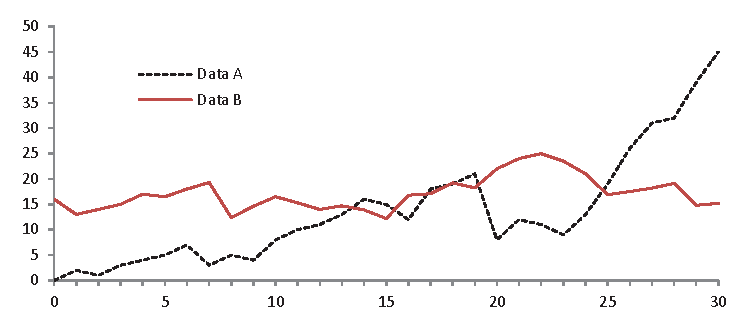
\includegraphics[width=\textwidth]{fig1.eps}
\caption{A figure caption is always placed below the illustration.
Please note that short captions are centered, while long ones are
justified by the macro package automatically.} \label{fig1}
\end{figure}

\begin{theorem}
This is a sample theorem. The run-in heading is set in bold, while
the following text appears in italics. Definitions, lemmas,
propositions, and corollaries are styled the same way.
\end{theorem}
%
% the environments 'definition', 'lemma', 'proposition', 'corollary',
% 'remark', and 'example' are defined in the LLNCS documentclass as well.
%
\begin{proof}
Proofs, examples, and remarks have the initial word in italics,
while the following text appears in normal font.
\end{proof}
For citations of references, we prefer the use of square brackets
and consecutive numbers. Citations using labels or the author/year
convention are also acceptable. The following bibliography provides
a sample reference list with entries for journal
articles~\cite{ref_article1}, an LNCS chapter~\cite{ref_lncs1}, a
book~\cite{ref_book1}, proceedings without editors~\cite{ref_proc1},
and a homepage~\cite{ref_url1}. Multiple citations are grouped
\cite{ref_article1,ref_lncs1,ref_book1},
\cite{ref_article1,ref_book1,ref_proc1,ref_url1}.

\subsubsection{Acknowledgements} Thanks to Professor Kosinski for answering some of my questions regarding his work and to Professor Wagner for assisting me during the seminar and writing of this paper.\cite{DUMMY:1}

%\printbibliography

%
% ---- Bibliography ----
%
% BibTeX users should specify bibliography style 'splncs04'.
% References will then be sorted and formatted in the correct style.
%

%
\bibliography{text/references}
% Bibliography
\bibliographystyle{splncs04}

\begin{thebibliography}{8}
\bibitem{ref_article1}
Author, F.: Article title. Journal \textbf{2}(5), 99--110 (2016)

\bibitem{ref_lncs1}
Author, F., Author, S.: Title of a proceedings paper. In: Editor,
F., Editor, S. (eds.) CONFERENCE 2016, LNCS, vol. 9999, pp. 1--13.
Springer, Heidelberg (2016). \doi{10.10007/1234567890}

\bibitem{ref_book1}
Author, F., Author, S., Author, T.: Book title. 2nd edn. Publisher,
Location (1999)

\bibitem{ref_proc1}
Author, A.-B.: Contribution title. In: 9th International Proceedings
on Proceedings, pp. 1--2. Publisher, Location (2010)

\bibitem{ref_url1}
LNCS Homepage, \url{http://www.springer.com/lncs}. Last accessed 4
Oct 2017
\end{thebibliography}
\end{document}
